%\frenchspacing
\usepackage{babel}
\usepackage[utf8]{inputenc}
\usepackage[T1]{fontenc}
%\usepackage[T1,mtbold,lucidacal,mtplusscr,subscriptcorrection]{mathtime}
\usepackage{times}
\usepackage[pdftex]{graphicx}
\usepackage{color}
%\usepackage{palatino}
\usepackage[pdftex,colorlinks=true,citecolor=black,bookmarks=true,
            pagecolor=black,linkcolor=black,menucolor=black,
            urlcolor=black]{hyperref}
\usepackage{amsmath,amsfonts,amssymb}
\usepackage[small,bf,up,margin=10pt]{caption} % Changes caption appearence
\usepackage{eufrak}
\usepackage{amsbsy}
\usepackage{eucal}
\usepackage{subfigure}
\usepackage{longtable}
\usepackage{url}
\RequirePackage{moreverb}
\RequirePackage{listings}
\urlstyle{same}
\usepackage[authoryear,round]{natbib}
\bibliographystyle{apalike}

\lstloadlanguages{[visual]C++,matlab}
\lstset{basicstyle=\normalsize,columns=fullflexible,frame=lines}

% Fix overflow
\pretolerance=150
\tolerance=150
\setlength{\emergencystretch}{3em}

% Orphan control
\widowpenalty=1000
\clubpenalty=1000
\raggedbottom


% Matlab code syntax highlight
\usepackage[framed]{mcode}
%\renewenvironment{verbatim}{\begin{lstlisting}}{\end{lstlisting}}

% Set cover background picture
\usepackage{eso-pic}
  \newcommand\BackgroundPic{
    \put(0,0){
    \parbox[b][\paperheight]{\paperwidth}{%
    \vfill
    \centering
    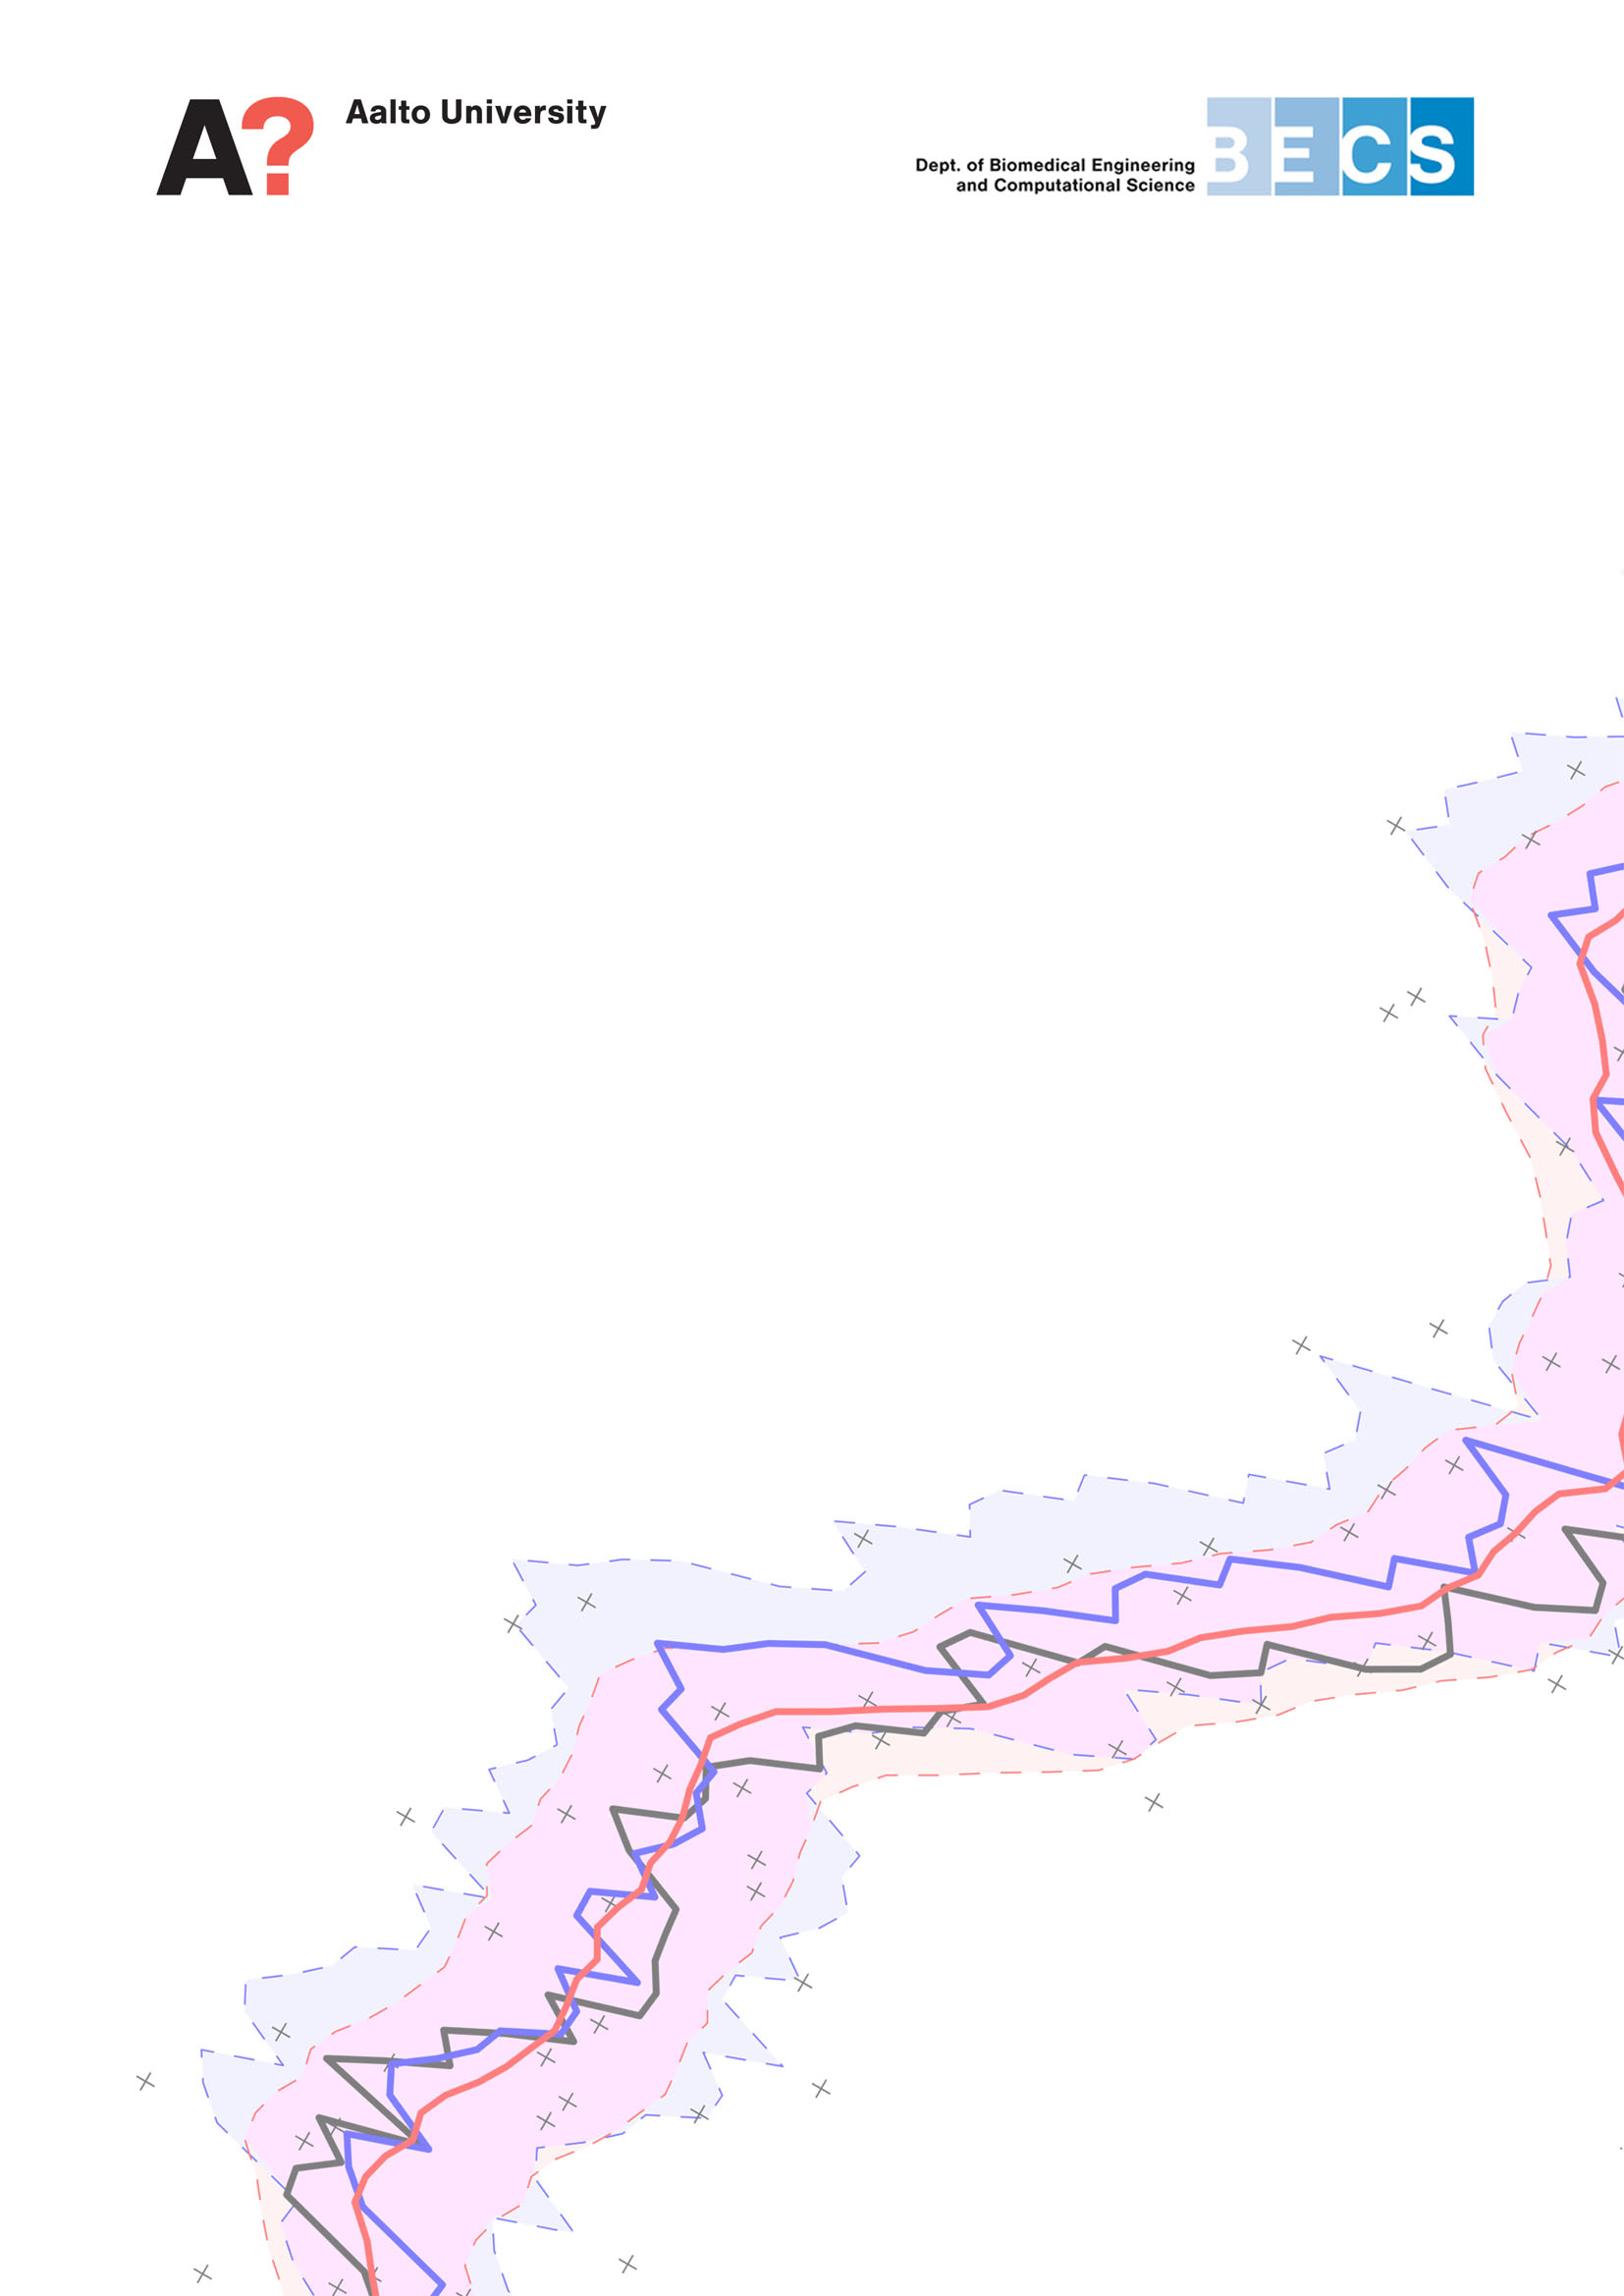
\includegraphics[width=\paperwidth,height=\paperheight,
      keepaspectratio]{pics/cover}%
    \vfill
  }}}



%\oddsidemargin 1cm    %   Note \oddsidemargin = \evensidemargin
%\evensidemargin 1cm
%\marginparwidth 0.2 true cm
%\topmargin -1.25cm
%\addtolength{\headsep}{0.25in}
%\textheight 21.5 true cm       % Height of text (including footnotes & figures)
%\textwidth 14 true cm        % Width of text line.

\usepackage{multirow}

% Headers
\usepackage{fancyhdr}
\pagestyle{fancy}
%\lhead{\textit{B.Sc. thesis draft \today}}
\lhead{\footnotesize \textsf \leftmark}
\chead{}
\rhead{}
\lfoot{}
\cfoot{\thepage}
\rfoot{}
\renewcommand{\headrulewidth}{0.5mm}
%\renewcommand{\footrulewidth}{0.5mm}

\pdfinfo{            
          /Title      (EFK/UKF toolbox for Matlab)
          /Author     (Jouni Hartikainen, Arno Solin, Simo Särkkä)
          /Keywords   (Kalman filter Extended Unscented optimal filtering)
}


%\newtheorem{Lemma}{Lemma}
%\newtheorem{Definition}{Definition}
%\DeclareMathOperator{\Poisson}{Poisson}
%\DeclareMathOperator{\GP}{\mathcal{GP}}
%\DeclareMathOperator{\Kfu}{\mathbf{K}_{f,u}}
%\DeclareMathOperator{\Kuf}{\mathbf{K}_{u,f}}
%\DeclareMathOperator{\Kff}{\mathbf{K}_{f,f}}
%\DeclareMathOperator{\Kfa}{\mathbf{K}_{f,\ast}}
%\DeclareMathOperator{\Kaf}{\mathbf{K}_{\ast,f}}
%\DeclareMathOperator{\Kaa}{\mathbf{K}_{\ast,\ast}}
%\DeclareMathOperator{\Kuu}{\mathbf{K}_{u,u}}
%\DeclareMathOperator{\Kau}{\mathbf{K}_{\ast,u}}
%\DeclareMathOperator{\Qff}{\mathbf{Q}_{f,f}}
%\DeclareMathOperator{\Qaa}{\mathbf{Q}_{\ast,\ast}}
%\DeclareMathOperator{\Qfa}{\mathbf{Q}_{f,\ast}}
%\DeclareMathOperator{\Qaf}{\mathbf{Q}_{\ast,f}}
%\DeclareMathOperator{\x}{\mathbf{x}}
%\DeclareMathOperator{\f}{\mathbf{f}}
%\DeclareMathOperator{\y}{\mathbf{y}}
%\DeclareMathOperator{\uu}{\mathbf{u}}
%\DeclareMathOperator{\LL}{\mathbf{\Lambda}}
%\DeclareMathOperator{\bb}{\mathbf{b}}

%\newcommand{\bm}{\mathbf}

\providecommand\figurename{Figure}
\providecommand\tablename{Table}
\providecommand\partname{Part}
\providecommand\appendixname{Appendix}
\providecommand\equationname{Eq\-ua\-tion}
%\providecommand\Itemname{item}
\providecommand\chaptername{chapter}
%\providecommand\sectionname{section}
\providecommand\subsectionname{section}
\providecommand\subsubsectionname{section}
%\providecommand\paragraphname{paragraph}
%\providecommand\theoremname{Theorem}


%%%%%%%%%%%%%%%%%%%%%%%%%%%%%%%%%%%%%%%%%
%
% macros begin
%
%%%%%%%%%%%%%%%%%%%%%%%%%%%%%%%%%%%%%%%%%
\renewcommand{\vec}[1]{\mathbf{#1}}
\newcommand{\set}[1]{\mathcal{#1}}
\newcommand{\alg}[1]{\mathscr{#1}}
\newcommand{\spc}[1]{\mathbb{#1}}
\newcommand{\ope}[1]{\EuScript{#1}}
\newcommand{\mea}[1]{#1}

\renewcommand{\vec}[1]{\mathbf{#1}}
\newcommand{\mat}[1]{\mathbf{#1}}
%\renewcommand{\vec}[1]{#1}
%\newcommand{\mat}[1]{#1}
\newcommand{\V}[1]{\mathbf{#1}}


\newcommand{\diff}[0]{\mathrm{d}}
%\newcommand{\diff}[0]{d}
%\newcommand{\B}[0]{\mathrm{\beta}}
%\newcommand{\Dt}[0]{\partial t}
\newcommand{\Dt}[0]{\delta t}
\newcommand{\Dx}[0]{\delta \vec{x}}
\newcommand{\Eg}[0]{\EuScript{E}}
\newcommand{\T}[0]{\mathsf{^T}}

\newcommand{\vectheta}[0]{\boldsymbol{\theta}}
\newcommand{\vecalpha}[0]{\boldsymbol{\alpha}}
\newcommand{\vecbeta}[0]{\boldsymbol{\beta}}
\newcommand{\veceta}[0]{\boldsymbol{\eta}}
\newcommand{\vecmu}[0]{\boldsymbol{\mu}}
\newcommand{\vecsigma}[0]{\boldsymbol{\sigma}}

%\DeclareMathOperator{\tr}{trace}
\DeclareMathOperator{\tr}{tr}
\DeclareMathOperator{\diag}{diag}
\DeclareMathOperator{\chol}{chol}
\DeclareMathOperator{\dchol}{dchol}
\DeclareMathOperator{\Cov}{Cov}
\DeclareMathOperator{\Var}{Var}
\DeclareMathOperator{\E}{E}
\DeclareMathOperator{\N}{N}
\DeclareMathOperator{\gammad}{Gamma}
\DeclareMathOperator{\expd}{Exp}
\DeclareMathOperator{\sech}{sech}
\DeclareMathOperator{\dt}{\Delta t}
\DeclareMathOperator{\dtk}{\Delta t_k}


\newcommand{\balpha}[0]{\boldsymbol{\alpha}}
\newcommand{\bbeta}[0]{\boldsymbol{\beta}}
\newcommand{\btheta}[0]{\boldsymbol{\theta}}
\newcommand{\bphi}[0]{\boldsymbol{\phi}}
\newcommand{\bmu}[0]{\boldsymbol{\mu}}
\newcommand{\bSigma}[0]{\boldsymbol{\Sigma}}
\newcommand{\blambda}[0]{\boldsymbol{\lambda}}
\newcommand{\brho}[0]{\boldsymbol{\rho}}
\newcommand{\bGamma}[0]{\boldsymbol{\Gamma}}

%\newtheorem{example}{Example}[section]
%\newtheorem{definition}{Definition}[section]
%\newtheorem{theorem}{Theorem}[section]
%\newtheorem{lemma}{Lemma}[section]
%\newtheorem{corollary}{Corollary}[section]
%\newtheorem{property}{Property}[section]

%\newtheorem{algorithm}{Algorithm}[chapter]
%\newtheorem{example}{Example}[chapter]
%\newtheorem{definition}{Definition}[chapter]
%\newtheorem{theorem}{Theorem}[chapter]
%\newtheorem{lemma}{Lemma}[chapter]
%\newtheorem{corollary}{Corollary}[chapter]
%\newtheorem{property}{Property}[chapter]
%\newtheorem{remark}{Remark}[chapter]

%%%%%%%%%%%%%%%%%%%%%%%%%%%%%%%%%%%%%%%%%
%
% macros end
%
%%%%%%%%%%%%%%%%%%%%%%%%%%%%%%%%%%%%%%%%%

% Lists
\newenvironment{boxlist1}{
  \begin{list}{}{\leftmargin=2pt}}{ % \leftmargin=0pt,
    % $\bullet$  ,\parsep=0pt
  \end{list}}
\newenvironment{boxlist2}{
  \begin{list}{-}{\itemsep=-1pt,\topsep=0pt,\setlength{\leftmargin}{8pt}}}{
    % 
  \end{list}}

\title{{\Huge Optimal Filtering \\with Kalman Filters and Smoothers} \\
  a Manual for the Matlab toolbox EKF/UKF \\
  {\normalsize Version~1.3}}

\author{Jouni Hartikainen, Arno Solin, and Simo Särkkä\\
Department of Biomedical Engineering and Computational Science,\\
Aalto University School of Science,\\
P.O.Box 1100, FI-00076 AALTO, Espoo, Finland \\
{\it jouni.hartikainen@aalto.fi, arno.solin@aalto.fi, simo.sarkka@aalto.fi}\vspace{-.5\baselineskip}}
%\date{}


\newenvironment{demo1}{\noindent\textbf{demo\_2input:}\begin{quote}\small\itshape}
{\end{quote}}

\newenvironment{example}{\small\begin{verbatim}}
{\end{verbatim}}

\newenvironment{demo2}{\noindent\textbf{demo\_2ingp:}\begin{quote}\small\itshape}
{\end{quote}}


